\section{Technologische Grundlagen}\label{zurhauptdatei}

\subsection{Docker: Grundlagen und Anwendung}\label{präambel}
Docker ist eine Open-Source-Plattform, die zur Containerisierung von Anwendungen dient. Anstatt Software direkt auf einem Betriebssystem zu installieren, verpackt Docker Anwendungen in Container, die alles enthalten, was für ihre Ausführung benötigt wird. Dies macht die Bereitstellung und den Betrieb von Software deutlich einfacher und effizienter. Seit der Veröffentlichung ist Docker der neue Standard geworden für private und kommerzielle Zwecke, die heutzutage nicht mehr wegzudenken sind. Docker basiert auf mehreren zentralen Komponenten, darunter Docker-Images, die als Baupläne für Container dienen und die gesamte Software-Umgebung definieren, sowie Docker-Container, die laufende Instanzen dieser Images sind und die Anwendung tatsächlich ausführen. Zusätzlich ermöglichen Docker-Netzwerke die Kommunikation zwischen verschiedenen Containern, was die Interaktion zwischen Diensten erleichtert, ohne dass diese direkt auf dem Host-System installiert sein müssen.

Einer der größten Vorteile von Docker ist seine Portabilität. Docker-Container können auf jedem System ausgeführt werden, das Docker unterstützt, sei es lokal, in der Cloud oder in einer Testumgebung. Dadurch wird die Anwendungsbereitstellung über verschiedene Umgebungen hinweg vereinfacht. Ein weiterer Vorteil ist die Ressourceneffizienz. Im Gegensatz zu virtuellen Maschinen, die ein vollständiges Betriebssystem für jede Anwendung benötigen, teilen sich Docker-Container das Host-Betriebssystem, was sie deutlich ressourcenschonender macht. Darüber hinaus bietet Docker eine hervorragende Skalierbarkeit, da Anwendungen leicht auf mehrere Container verteilt werden können, um Lasten zu verteilen und die Leistung zu optimieren. Ein weiterer Pluspunkt ist das schnelle Deployment, da Container in Sekunden gestartet und gestoppt werden können, was die Bereitstellungszeiten erheblich verkürzt.

In unserem Projekt haben wir Docker genutzt, um verschiedene Dienste voneinander zu trennen und die Anwendung flexibel zu skalieren. Wir haben beispielsweise den Webserver, bestehend aus Apache und CGI, in einem eigenen Container betrieben, um ihn von anderen Diensten zu isolieren. Die Datenbank, MariaDB, wurde in einem separaten Container ausgeführt, um die Datenverwaltung von der Anwendungslogik zu trennen. Zusätzlich haben wir Redis als Caching-Dienst und zur Sessionverwaltung in einem weiteren Container eingesetzt, um die Leistung unserer Anwendung zu verbessern. Zusätzlich haben wir einen Work-Container für die Lasttests. Durch diese Aufteilung konnten wir die Anwendung effizient skalieren und Lasttests durchführen, ohne uns um Abhängigkeiten oder Konflikte zwischen den Diensten sorgen zu müssen. Docker hat die Entwicklung und das Deployment unserer Anwendung erheblich vereinfacht und beschleunigt.

\subsection{Das ISO/OSI-Modell}\label{zitierstil}
Das ISO/OSI-Modell ist ein wichtiges Referenzmodell für die Netzwerkkommunikation und besteht aus sieben Schichten, die beschreiben, wie Daten zwischen verschiedenen Systemen übertragen werden. In unserem Projekt, einer ToDo-Liste, die auf Docker-Containern basiert, nutzen wir dieses Modell, um die Kommunikation zwischen den verschiedenen Komponenten wie dem HAProxy-Load-Balancer, dem Apache-Webserver, der MariaDB-Datenbank und dem Redis-Caching-System zu organisieren. Jede dieser Komponenten hat eine spezifische Funktion: Der HAProxy nimmt die eingehenden HTTP-Anfragen entgegen und leitet sie an die Apache-Server weiter, die die Anfragen bearbeiten und die Antworten zurückliefern. MariaDB speichert die Daten der ToDo-Liste, und Redis übernimmt die Sessionverwaltung, um Benutzeranmeldungen effizient zu handhaben. Die Kommunikation zwischen diesen Komponenten erfolgt über verschiedene Schichten des OSI-Modells, was eine klare Trennung und effiziente Verwaltung der Netzwerkprozesse ermöglicht. Auf der Anwendungsschicht laufen beispielsweise die HTTP-Anfragen zwischen dem Client und dem HAProxy sowie die CGI-Skripte für die ToDo-Liste auf den Apache-Servern. Die Transportschicht sorgt mit TCP-Verbindungen durch die Bi-direktionale Kommunikation für eine zuverlässige Verbindung zwischen HAProxy und den Apache-Servern, während die Internetschicht die Datenpakete über IP-Adressen im Docker-Netzwerk routet. In der Sicherungsschicht werden Ethernet-Frames verwendet, um die Daten innerhalb des Netzwerks zuverlässig zu übertragen. Durch diese klare Strukturierung können wir die Kommunikation zwischen den Komponenten effizient verwalten und sicherstellen, dass die Datenübertragung reibungslos funktioniert.
\begin{figure}[ht!]
        \centering
        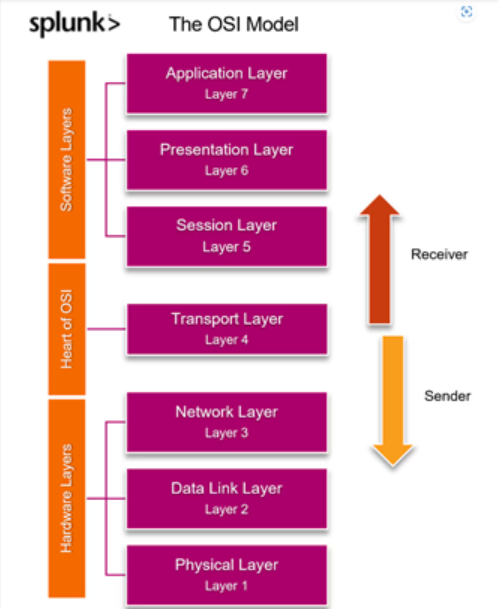
\includegraphics[width=0.65\textwidth]{src/abbildungen/osi.png}
        \caption{OSI-Modell}
\end{figure}
\FloatBarrier
\begin{figure}[ht!]
        \centering
        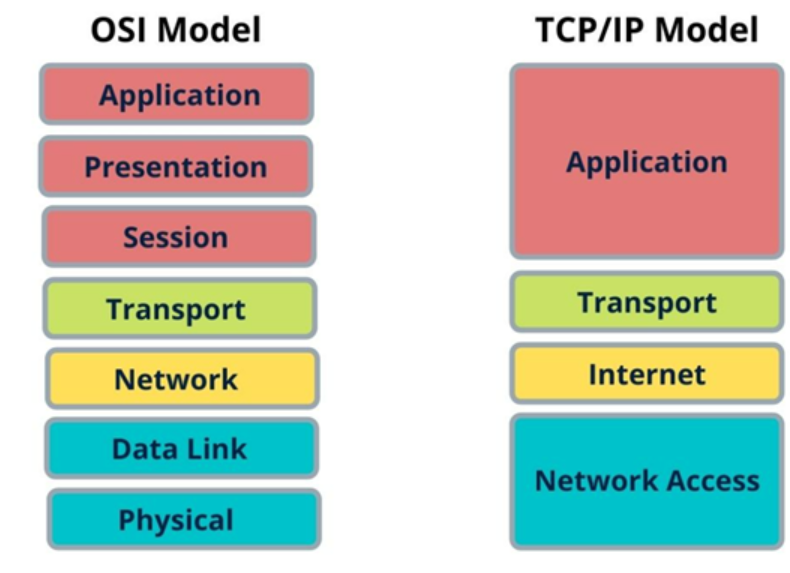
\includegraphics[width=0.65\textwidth]{src/abbildungen/tcp.png}
        \caption{OSI-Modell und TCP/IP Modell}
\end{figure}
\FloatBarrier

Die erste Schicht, der Physical Layer, bezieht sich auf die physische Übertragung von Daten.
In unserem Projekt läuft die gesamte Infrastruktur auf einem Host-System, das entweder über ein kabelgebundenes Netzwerk (Ethernet) oder eine WLAN-Verbindung mit dem Internet verbunden ist. Innerhalb der Docker-Umgebung existiert jedoch keine physische Verbindung, sondern eine virtuelle Netzwerkarchitektur, die auf der Netzwerkinfrastruktur des Host-Systems aufbaut. Dadurch können die Container miteinander kommunizieren, ohne dass eine direkte physische Verbindung zwischen ihnen besteht.

Die zweite Schicht, der Data Link Layer, sorgt für die fehlerfreie Übertragung von Datenpaketen innerhalb eines lokalen Netzwerks. In unserem Projekt ermöglicht Docker dies durch virtuelle Netzwerkbrücken wie docker0, die eine sichere interne Kommunikation zwischen den Containern gewährleisten. Diese Netzwerkbrücken verwalten virtuelle MAC-Adressen und steuern den Datenfluss zwischen den Containern. Da in virtuellen Netzwerken keine echten Kollisionen auftreten, nutzt Docker Switching-Mechanismen zur Datenübertragung.

Die dritte Schicht, der Network Layer, ist für die Adressierung und das Routing von Datenpaketen verantwortlich. In unserem Projekt erhält jeder Docker-Container eine eigene IP-Adresse, die zur Kommunikation mit anderen Containern genutzt wird. Der HAProxy-Load-Balancer verteilt eingehende Anfragen anhand dieser IP-Adressen an verschiedene Backend-Dienste. Die gesamte Kommunikation zwischen Webserver, Datenbank und Caching-System erfolgt innerhalb eines privaten Docker-Netzwerks, das eine sichere und isolierte Umgebung für den Datenaustausch bietet.

Die vierte Schicht, der Transport Layer, stellt eine zuverlässige Ende-zu-Ende-Kommunikation sicher und entscheidet, ob eine Verbindung verbindungsorientiert (z. B. TCP) oder verbindungslos (z. B. UDP) aufgebaut wird. In unserem Projekt nutzen wir ausschließlich TCP (Transmission Control Protocol), da unser System eine stabile und fehlerfreie Datenübertragung benötigt. Der Apache-Webserver empfängt HTTP-Anfragen über TCP und leitet diese an die Datenbank oder das Caching-System weiter. Auch MariaDB nutzt TCP für die Übertragung von SQL-Abfragen, um eine zuverlässige Kommunikation mit der Anwendung sicherzustellen. Redis setzt ebenfalls auf TCP, um schnelle und stabile Anfragen zwischen dem Caching-System und der Anwendung zu ermöglichen. Besonders wichtig in dieser Schicht ist der Three-Way-Handshake (SYN, SYN-ACK, ACK), der für jede neue TCP-Verbindung zwischen Client und Server durchgeführt wird. Dieser Mechanismus sorgt dafür, dass die Datenübertragung zuverlässig ist und keine Pakete verloren gehen.

Die fünfte Schicht, der Session Layer, ist für die Verwaltung und Aufrechterhaltung von Sitzungen zwischen Client und Server verantwortlich. In unserem Projekt spielt Redis eine wichtige Rolle bei der Sitzungsverwaltung, indem es temporäre Login-Informationen speichert. Dadurch bleibt ein Nutzer auch nach mehreren Anfragen authentifiziert, ohne sich erneut anmelden zu müssen. Allerdings übernimmt Redis hier eher eine anwendungsbezogene Funktion, während klassische Sitzungsprotokolle wie Telnet oder SQL-Sitzungen direkte Beispiele für den Session Layer wären.

Die sechste Schicht, der Presentation Layer, sorgt für die Umwandlung, Komprimierung und Verschlüsselung von Daten. Zudem sorgt HTTPS (TLS/SSL) für eine sichere Übertragung, indem es die Daten verschlüsselt, sodass sie nicht von Dritten abgefangen werden können. Die eigentliche Verschlüsselung findet auf der Transportebene durch TLS statt, wird aber oft mit der Präsentationsebene in Verbindung gebracht.

Die siebte Schicht, der Application Layer, ist die Schnittstelle zwischen dem Nutzer und der Anwendung. In unserem ToDo-Listen-Projekt erfolgt der Zugriff über eine Webseite mit HTML, CSS, JavaScript und CGI-Skripten. Der Apache-Webserver verarbeitet die eingehenden Anfragen und sendet die entsprechenden Antworten an den Client. REST-APIs ermöglichen die Kommunikation zwischen der Benutzeroberfläche und der Datenbank, indem sie strukturierte Anfragen und Antworten über HTTP bereitstellen.
